\section{Experiments}

We use the crypto data described above to train and test the performance of the different models. Due to computational limitations, we take the last 100k time steps with 90k time steps for training and the last 10k used as a test set. Training hyperparameters were tuned manually to find a reasonable best-performing combination.

\subsection{Results}

\begin{figure}[H]
	\centering
	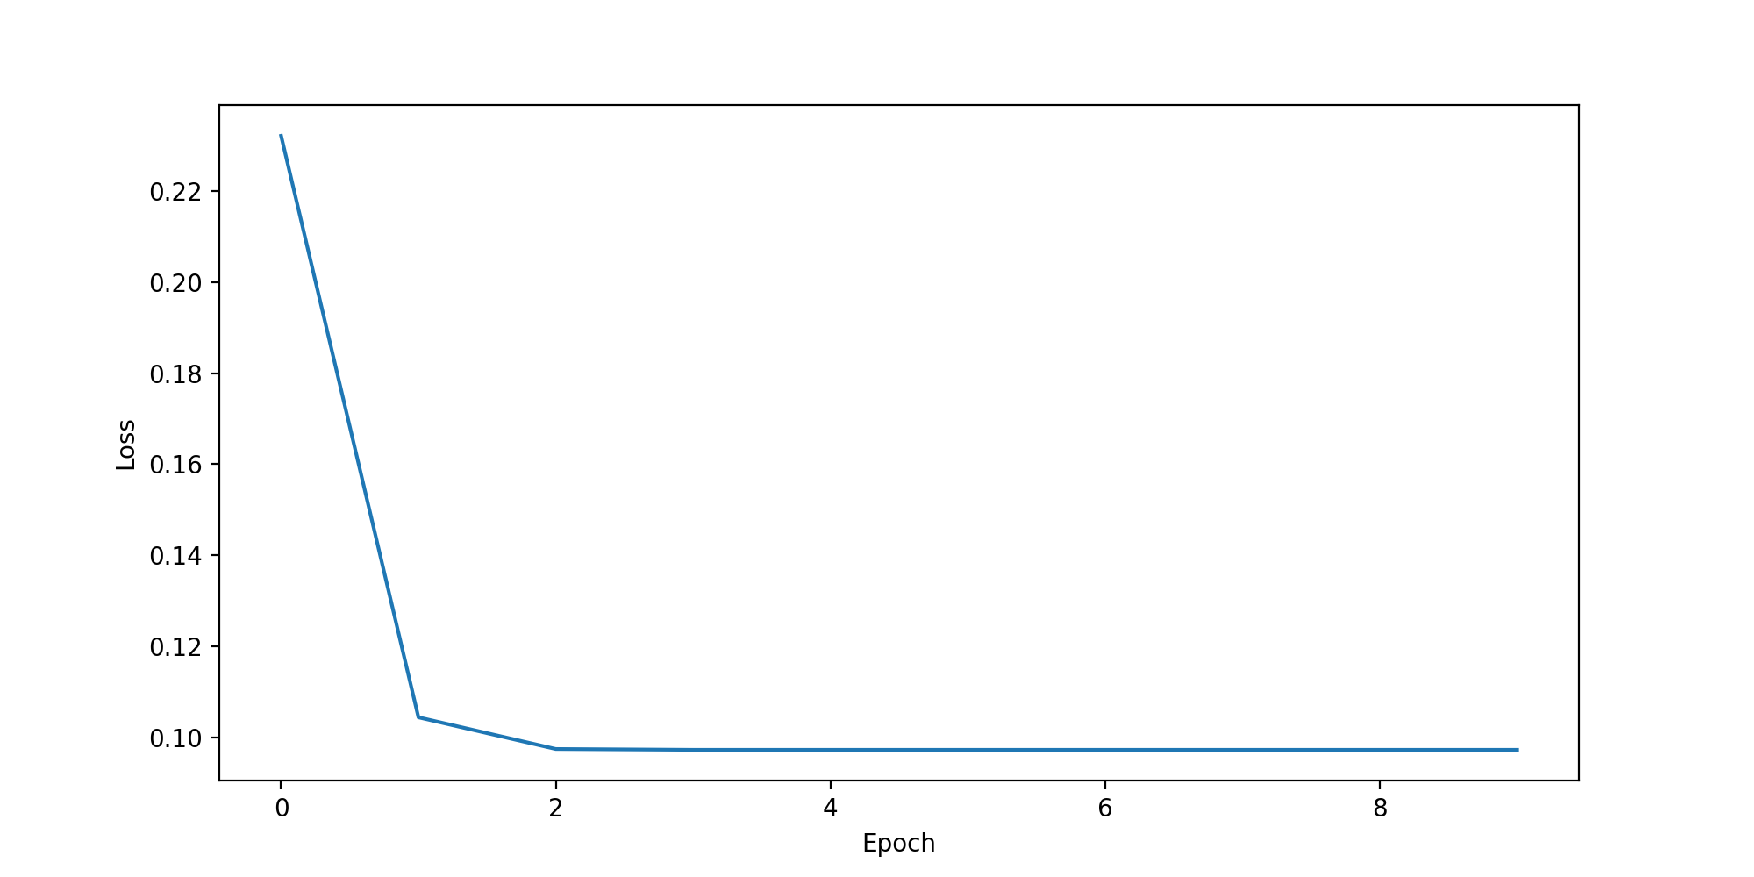
\includegraphics[width=\linewidth]{../../figures/vanilla_lstm_training_loss.pdf}
	\caption{Training loss of baseline LSTM model}
	\label{fig:lstm_loss}
\end{figure}

\begin{table}[H]
	\centering
	\begin{tabular}{|c|c|c|c|c|}
	\hline
	Model & Optimzier & Learning Rate & Momentum & MSE \\
	\hline
	LSTM & SGD & 0.0001 & 0.9 & 0.0030 \\
	Additive & & & & \\
	Sequential & & & & \\
	\hline
	\end{tabular}
	\caption{Hyperparameters for best performing model with average MSE on validation set}
	\label{tab:results_summary}
\end{table}